%\documentclass[landscape,a0b,final,a4resizeable]{a0poster}
\documentclass[landscape,a0b,final]{a0poster}
%\documentclass[portrait,a0b,final,a4resizeable]{a0poster}
%\documentclass[portrait,a0b,final]{a0poster}
%%% Option "a4resizeable" makes it possible to resize the
%   poster by the command: psresize -pa4 poster.ps poster-a4.ps
%   For final printing, please remove option "a4resizeable" !!

\usepackage{epsfig}
\usepackage{multicol}
\usepackage{pstricks,pst-grad}
\usepackage{graphicx,psfrag}
\usepackage{graphics}
\usepackage{amsmath}
\usepackage{amsthm}
\usepackage{amsfonts}

\newtheorem{example}{Example}
\newtheorem{assumption}{Assumption}
\newtheorem{definition}{Definition}
\newtheorem{theorem}{Theorem}
\newtheorem{lemma}{Lemma}


%%%%%%%%%%%%%%%%%%%%%%%%%%%5

\usepackage{eso-pic}
\usepackage{graphicx}
\usepackage{color}
\usepackage{type1cm}


%%%%%%%%%%%%%%%%%%%%%%%%%%%%%%%%%%%%%%%%%%%%%%%%%%%%
%%%               WaterMark                       %%%
%%%%%%%%%%%%%%%%%%%%%%%%%%%%%%%%%%%%%%%%%%%%%%%%%%%%
%\makeatletter
%  \AddToShipoutPicture{%
%    \setlength{\@tempdimb}{.5\paperwidth}%
%    \setlength{\@tempdimc}{.5\paperheight}%
%    \setlength{\unitlength}{1pt}%
%    \put(\strip@pt\@tempdimb,\strip@pt\@tempdimc){%
%      \makebox(0,0){\rotatebox{45}{\textcolor[gray]{0.15}{\includegraphics[width=120cm,angle=0]{SU_Seal_Card_pos.eps}}}}
%    }
%}
%\makeatother



%%%%%%%%%%%%%%%%%%%%%%%%%%%%%%%%%%%%%%%%%%%
% Definition of some variables and colors
%\renewcommand{\rho}{\varrho}
%\renewcommand{\phi}{\varphi}
\setlength{\columnsep}{3cm}
\setlength{\columnseprule}{2mm}
\setlength{\parindent}{0.0cm}



%%%%%%%%%%%%%%%%%%%%%%%%%%%%%%%%%%%%%%%%%%%%%%%%%%%%
%%%               Background                     %%%
%%%%%%%%%%%%%%%%%%%%%%%%%%%%%%%%%%%%%%%%%%%%%%%%%%%%

\newcommand{\background}[3]{
  \newrgbcolor{cgradbegin}{#1}
  \newrgbcolor{cgradend}{#2}
  \psframe[fillstyle=gradient,gradend=cgradend,
  gradbegin=cgradbegin,gradmidpoint=#3](0.,0.)(1.\textwidth,-1.\textheight)
}



%%%%%%%%%%%%%%%%%%%%%%%%%%%%%%%%%%%%%%%%%%%%%%%%%%%%
%%%                Poster                        %%%
%%%%%%%%%%%%%%%%%%%%%%%%%%%%%%%%%%%%%%%%%%%%%%%%%%%%

\newenvironment{poster}{
  \begin{center}
  \begin{minipage}[c]{0.98\textwidth}
}{
  \end{minipage} 
  \end{center}
}



%%%%%%%%%%%%%%%%%%%%%%%%%%%%%%%%%%%%%%%%%%%%%%%%%%%%
%%%                pcolumn                       %%%
%%%%%%%%%%%%%%%%%%%%%%%%%%%%%%%%%%%%%%%%%%%%%%%%%%%%

\newenvironment{pcolumn}[1]{
  \begin{minipage}{#1\textwidth}
  \begin{center}
}{
  \end{center}
  \end{minipage}
}



%%%%%%%%%%%%%%%%%%%%%%%%%%%%%%%%%%%%%%%%%%%%%%%%%%%%
%%%                pbox                          %%%
%%%%%%%%%%%%%%%%%%%%%%%%%%%%%%%%%%%%%%%%%%%%%%%%%%%%

%\newrgbcolor{lcolor}{0. 0. 0.80}
\newrgbcolor{lcolor}{1 1 1}
\newrgbcolor{gcolor1}{1. 1. 1.}
\newrgbcolor{gcolor2}{.80 .80 1.}

\newcommand{\pbox}[4]{
\psshadowbox[#3]{
\begin{minipage}[t][#2][t]{#1}
#4
\end{minipage}
}}



%%%%%%%%%%%%%%%%%%%%%%%%%%%%%%%%%%%%%%%%%%%%%%%%%%%%
%%%                myfig                         %%%
%%%%%%%%%%%%%%%%%%%%%%%%%%%%%%%%%%%%%%%%%%%%%%%%%%%%
% \myfig - replacement for \figure
% necessary, since in multicol-environment 
% \figure won't work

\newcommand{\myfig}[3][0]{
\begin{center}
  \vspace{1.5cm}
  \includegraphics[width=#3\hsize,angle=#1]{#2}
  \nobreak\medskip
\end{center}}

\newcommand{\myfigp}[3][0]{
\begin{center}
  \vspace{1.5cm}
  \includegraphics[width=#3\hsize]{#1}
  \includegraphics[width=#3\hsize]{#2}
  \nobreak\medskip
\end{center}}



%%%%%%%%%%%%%%%%%%%%%%%%%%%%%%%%%%%%%%%%%%%%%%%%%%%%
%%%                mycaption                     %%%
%%%%%%%%%%%%%%%%%%%%%%%%%%%%%%%%%%%%%%%%%%%%%%%%%%%%
% \mycaption - replacement for \caption
% necessary, since in multicol-environment \figure and
% therefore \caption won't work

%\newcounter{figure}
\setcounter{figure}{1}
\newcommand{\mycaption}[1]{
  \vspace{0.5cm}
  \begin{quote}
    {{\sc Figure} \arabic{figure}: #1}
  \end{quote}
  \vspace{1cm}
  \stepcounter{figure}
}



%%%%%%%%%%%%%%%%%%%%%%%%%%%%%%%%%%%%%%%%%%%%%%%%%%%%%%%%%%%%%%%%%%%%%%
%%% Begin of Document
%%%%%%%%%%%%%%%%%%%%%%%%%%%%%%%%%%%%%%%%%%%%%%%%%%%%%%%%%%%%%%%%%%%%%%

\begin{document}





\newrgbcolor{lightblue}{0. 0. 0.80}
\newrgbcolor{white}{1. 1. 1.}
\newrgbcolor{whiteblue}{1 1 1}
\newrgbcolor{red}{0.6431 0 0.1137}
\newrgbcolor{whitered}{0.6431 0 0.1137}




\begin{poster}

\background{0.6431 0 0.1137}{1. 1. 1.}{0.5}
\vspace*{2.5cm}
%%%%%%%%%%%%%%%%%%%%%
%%% Header
%%%%%%%%%%%%%%%%%%%%%
\begin{center}
\begin{pcolumn}{0.992}

\pbox{0.95\textwidth}{}{linewidth=4mm,framearc=0.3,linecolor=red,fillstyle=gradient,gradangle=0,gradbegin=white,gradend=white,gradmidpoint=1.0,framesep=1em}{

%%% DARPA-DSO logo
\begin{minipage}[c][4.5cm][c]{0.13\textwidth}
  \begin{center}
    
\includegraphics[width=13cm,angle=0]{Darpadsologo}
  \end{center}
\end{minipage}
%%% AA logo
\begin{minipage}[c][4.5cm][c]{0.14\textwidth}
  \begin{center}
    %\includegraphics[width=8cm,angle=0]{SU_Seal_Card_pos}
    \vspace{5mm}
    
\includegraphics[width=12cm,angle=0]{aalogo}
  \end{center}
\end{minipage}
%%% Title
\begin{minipage}[c][9cm][c]{0.46\textwidth}
  \begin{center}
    {\sc \Huge Cutoff Phenomena in Chaotic Dynamics}\\[10mm]
    {\Large Tzu-Chen Liang\\[7.5mm]
     Department of Aeronautics and Astronautics, Stanford University }
  \end{center}
\end{minipage}
%%% Stanford logo
\begin{minipage}[c][4.5cm][c]{0.10\textwidth}
  \begin{center}
    \hspace{2cm}
    \includegraphics[width=8cm,angle=0]{SU_Seal_Card_pos}
  \end{center}
\end{minipage}
%%% DynaRUM logo
\begin{minipage}[c][9cm][c]{0.17\textwidth}
  \begin{center}
    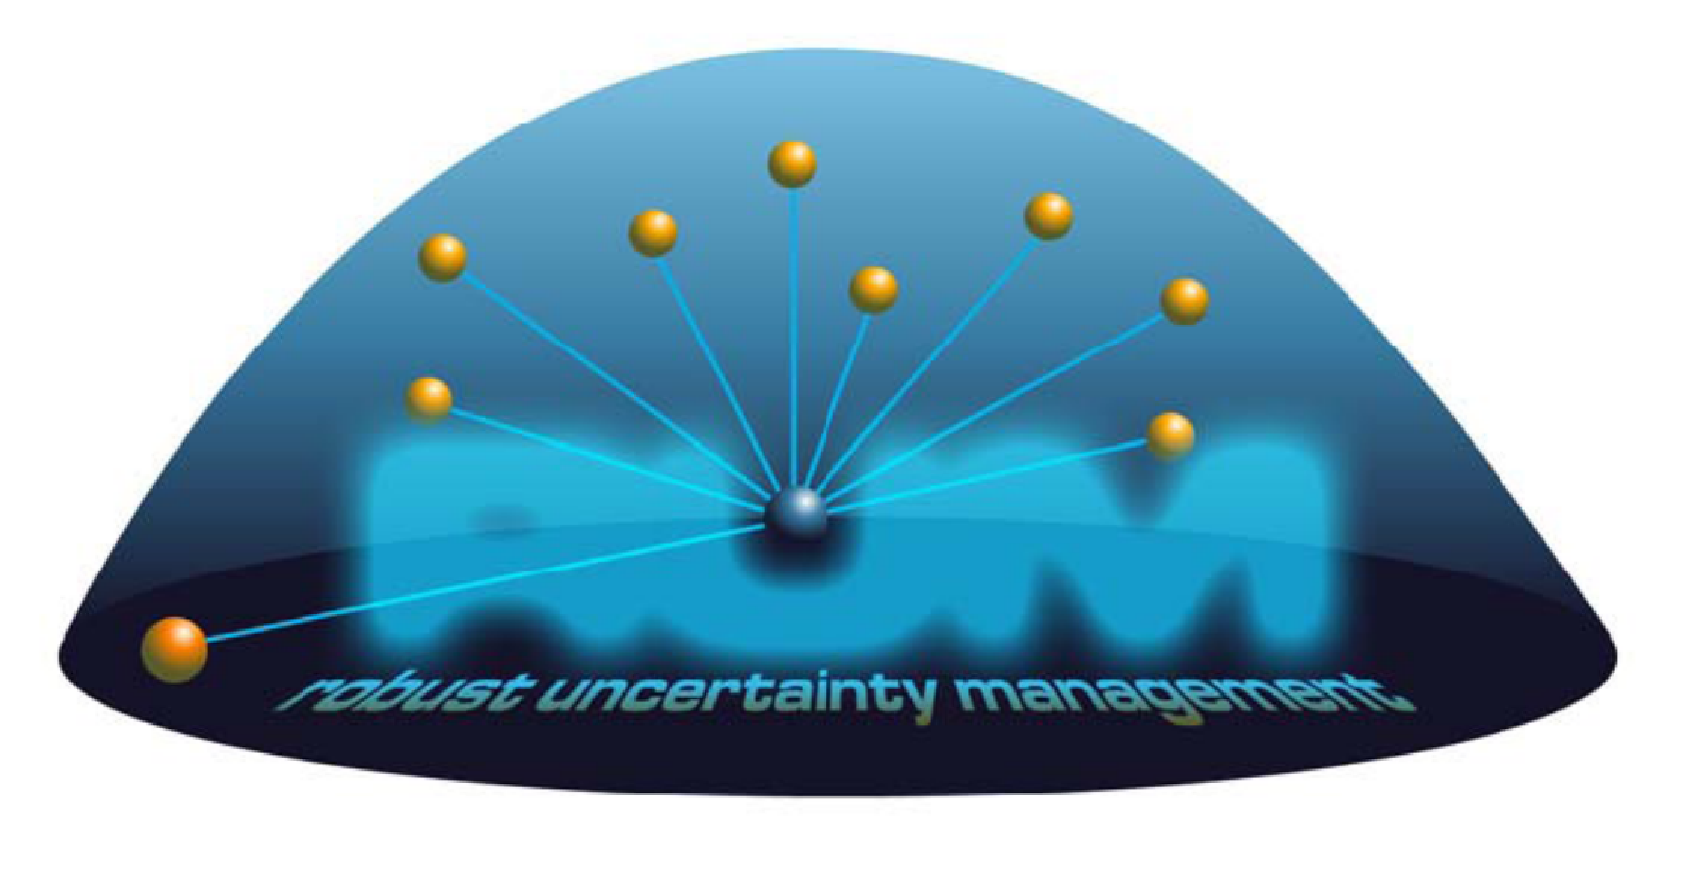
\includegraphics[width=15cm,angle=0]{Dynarumlogo}
  \end{center}
\end{minipage}
} 



%\pbox{0.95\textwidth}{}{linewidth=4mm,framearc=0.3,linecolor=red,fillstyle=gradient,gradangle=0,gradbegin=white,gradend=white,gradmidpoint=1.0,framesep=1em}{



%%% DARPA-DSO logo
%\begin{minipage}[c][4.5cm][c]{0.13\textwidth}
%  \begin{center}
%    
\includegraphics[width=12cm,angle=0]{Darpadsologo.eps}
%  \end{center}
%\end{minipage}
%%% Stanford logo
%\begin{minipage}[c][4.5cm][c]{0.1\textwidth}
%  \begin{center}
%    \includegraphics[width=8cm,angle=0]{SU_Seal_Card_pos.eps}
%  \end{center}
%\end{minipage}
%%% Title
%\begin{minipage}[c][9cm][c]{0.55\textwidth}
%  \begin{center}
%    {\sc \Huge Cutoff Phenomena in Chaotic Dynamics}\\[10mm]
%    {\Large Tzu-Chen Liang\\[7.5mm]
%     Department of Aeronautics and Astronautics, Stanford University }
%  \end{center}
%\end{minipage}
%%%% stanford logo
%\begin{minipage}[c][4.5cm][c]{0.1\textwidth}
%  \begin{center}
%    \includegraphics[width=8cm,angle=0]{SU_Seal_Card_pos.eps}
%  \end{center}
%\end{minipage}
%%% DynaRUM logo
%\begin{minipage}[c][9cm][c]{0.1\textwidth}
%  \begin{center}
%    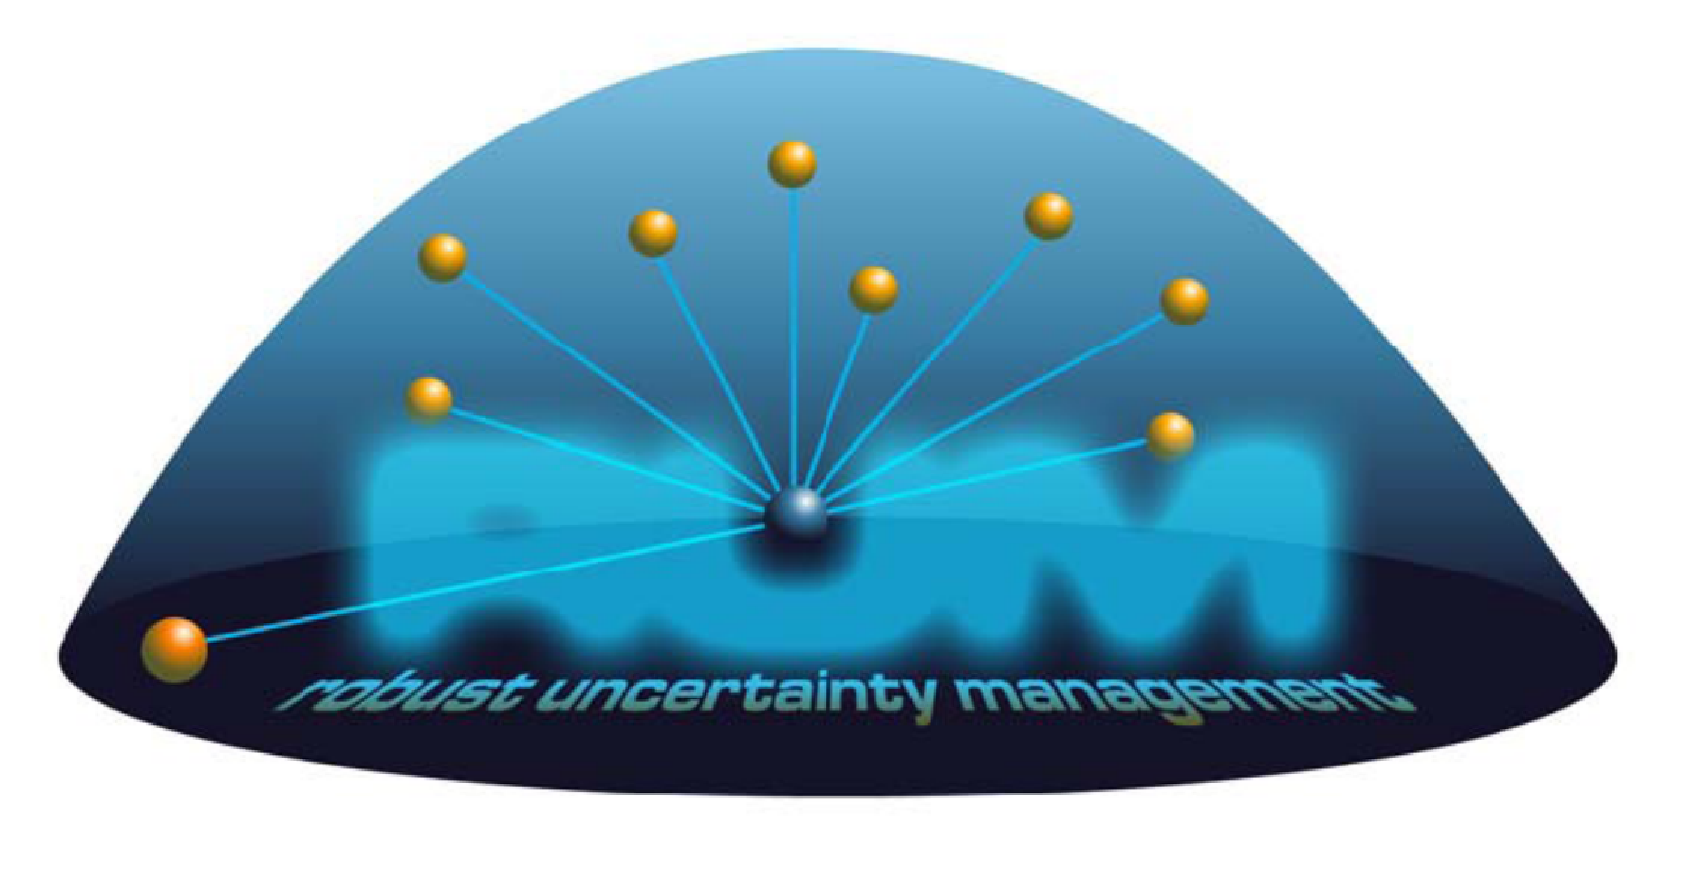
\includegraphics[width=12cm,angle=0]{Dynarumlogo.eps}
%  \end{center}
%\end{minipage}
%}




\end{pcolumn}
\end{center}


\vspace*{2cm}



%%%%%%%%%%%%%%%%%%%%%
%%% Content
%%%%%%%%%%%%%%%%%%%%%
%%%%%%%%%%%%%%%%%%%%%%%%%%%%%%%%
%Here is the 1st column
%%%%%%%%%%%%%%%%%%%%%%%%%%%%%%%%

\begin{center}
\begin{pcolumn}{0.32}
\pbox{0.9\textwidth}{65cm}{linewidth=4mm,framearc=0.1,linecolor=red,fillstyle=gradient,gradangle=0,gradbegin=white,gradend=white,gradmidpoint=1.0,framesep=1em}{

%%% Introduction
\begin{center}\pbox{0.8\textwidth}{}{linewidth=2mm,framearc=0.1,linecolor=red,fillstyle=gradient,gradangle=0,gradbegin=white,gradend=whitered,gradmidpoint=1.0,framesep=1em}{\begin{center}\bfseries{\large{Introduction}}\end{center}}\end{center}
\vspace{1.25cm}
%%%%%%%%%%%%%%%%%%%%%%%%%%%%%%%%%%%%%%%%%%%%%%%%%%%%%%%%%%%%%%%%%%%%%%%%%%%%%%%%%%%%%%%%%%%%%%%%
%Introduction begins here
%We relax the definition of cutoff phenomenon discovered in finite Markov chain simulations and apply it to the study of the evolving of a probability density function under tent map and logistic map. We then prove they both present cutoffs when a sequence of initial probability densities with ascending concentration is applied. Cutoffs also observed when a simple passive scalar function is advected by the same maps with small diffusion. We refer the above two as chaotic randomizing and chaotic mixing problems, and show they are close related. Numerical evidence of cutoff is also given for 2-D standard map. 
\begin{itemize}
 \item Prove the scalar measure of certainty/uncertainty can have a phase change(cutoff) under chaotic mapping. 
 \item Show the dual relation between chaotic mixing and chaotic randomizing problems.
 \item Numerical evidence of cutoff is provided for 2-D standard map with small diffution. 
\end{itemize}

\begin{tabular}{c|l}
  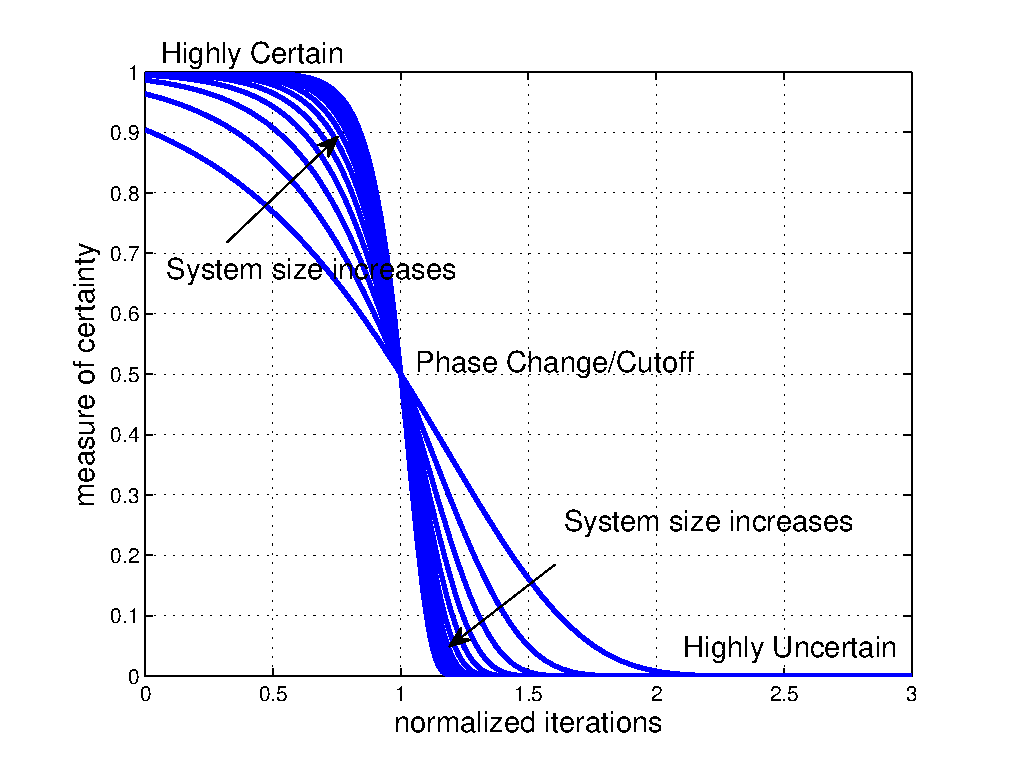
\includegraphics[width=0.55\hsize]{democutoffn}&
  \begin{minipage}[b]{0.43\hsize}
  \paragraph{The phase change of scalar measure of cetrainty}
  The scalar measure of certainty changes sharply from $1$ to $0$, which indicates the state of the system evolves from highly certain to highly uncertain. This tendency is reinforced when system size becomes larger, and thus presents a cutoff or a sharp phase change under the normalized plot.   
  \end{minipage}
\end{tabular}


%Introduction ends here
%%%%%%%%%%%%%%%%%%%%%%%%%%%%%%%%%%%%%%%%%%%%%%%%%%%%%%%%%%%%%%%%%%%%%%%%%%%%%%%%%%%%%%%%%%%%%%%%%




%%% Cutoff 
\vspace{0.7cm}\begin{center}\pbox{0.8\textwidth}{}{linewidth=2mm,framearc=0.1,linecolor=red,fillstyle=gradient,gradangle=0,gradbegin=white,gradend=whitered,gradmidpoint=1.0,framesep=1em}{\begin{center}\bfseries{\large{Cutoff Phenomenon}}\end{center}}\end{center}\vspace{1cm}
%%%%%%%%%%%%%%%%%%%%%%%%%%%%%%%%%%%%%%%%%%%%%%%%%%%%%%%%%%%%%%%%%%%%%%%%%%%%%%%%%%%%%%%%%%%%%%%%
%section begins here
We state the definition of a cutoff given by Diaconis in
\cite{Diaconis2005}. Assume that, to any finite set $\Omega$ and any
pair of probability measures $\omega$, $\bar{\omega}$ on $\Omega$ is associated
a real number $D(\omega,\bar{\omega})$ such that $D(\omega,\bar{\omega})\in [0,1]$,
%\begin{eqnarray}
$\max_{\Omega,\omega,\bar{\omega}} D(\omega,\bar{\omega}) = 1$, 
%\end{eqnarray}
and $D(\omega,\bar{\omega})=0$ if and only if $\bar{\omega}=\omega$. Consider a sequence of
(finite) probability spaces $(\Omega_n,\bar{\omega}_n)$, $n=1,2,...$, each
equipped with a sequence of probability measure $\omega^k_n$,
$l=0,1,...$, such that
%\begin{eqnarray}
$\lim_{k \rightarrow \infty} D(\omega_n,\bar{\omega}_n)=0$.
%\end{eqnarray}
The definition of a cutoff is,

\begin{definition}
\label{cutoffdefinition}
(Diaconis) A family $(\Omega_n,\bar{\omega}_n, (\omega^k_n)_{k=0,1,...})_{n=1,2,...}$
presents a D-cutoff if there exists a sequence $(t_n)$ of positive
reals such that, for any $\epsilon \in(0,1)$,
\begin{enumerate}
  \item $\lim_{k \rightarrow \infty}D(\omega^{k_n}_n,\bar{\omega}_n) = 0 \mbox{ if }
  k_n>(1+\epsilon)t_n$
  \item $\lim_{k \rightarrow \infty}D(\omega^{k_n}_n,\bar{\omega}_n) = 1 \mbox{ if }
  k_n<(1-\epsilon)t_n $
\end{enumerate}
\end{definition}

In the next section, we need to relax the definition and set $\Omega_n$ to be infinite. We say that a family $(\Omega_n,\bar{\omega}_n, (\omega^k_n)_{k=0,1,...})_{n=1,2,...}$ presents a D-cutoff in the relaxed sense if it satisfies definition \ref{cutoffdefinition} but $\Omega_n$ is infinite. 

\begin{example} \textbf{Random walk on an $n$-dimensional hypercube}
 
\vspace{0.3cm}
\begin{tabular}{c|l}
  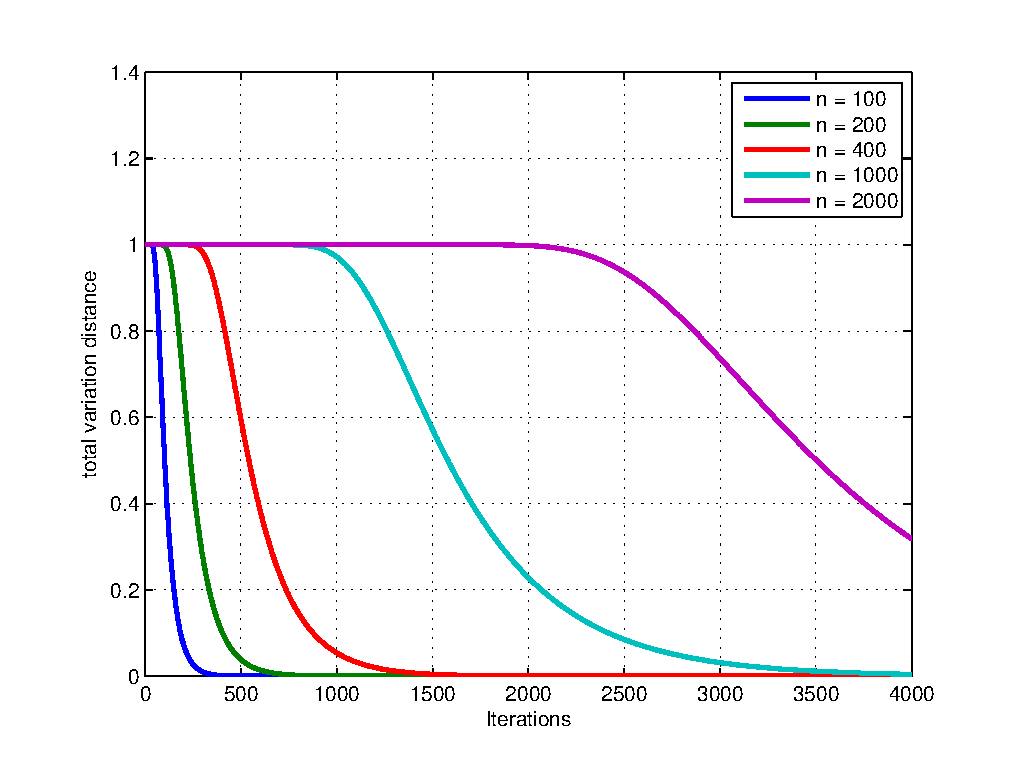
\includegraphics[width=0.4\hsize]{rdwalk.eps} &
\begin{minipage}[b]{0.58\hsize}
A particle starts at $\mathbf{0}$ and moves to one of its nearest neighbors (or stays fixed) with equal probability at each step.
\vspace{-1cm}
\paragraph{Total Variation Distance}
  \begin{eqnarray*}
   \|\omega^k - \bar{\omega}\|_{TV} = \frac{1}{2}\sum_{i=1}^n |\omega_i^k-\bar{\omega}_i |= \frac{1}{2}\sum_{i=1}^n |f_i^k-1|\bar{\omega}_i
  \end{eqnarray*}
  where $f^k_i = \omega_i^k/\bar{\omega}_i$. $f$ is the density of $\omega$ with respect to $\bar{\omega}$.
\end{minipage}
\\
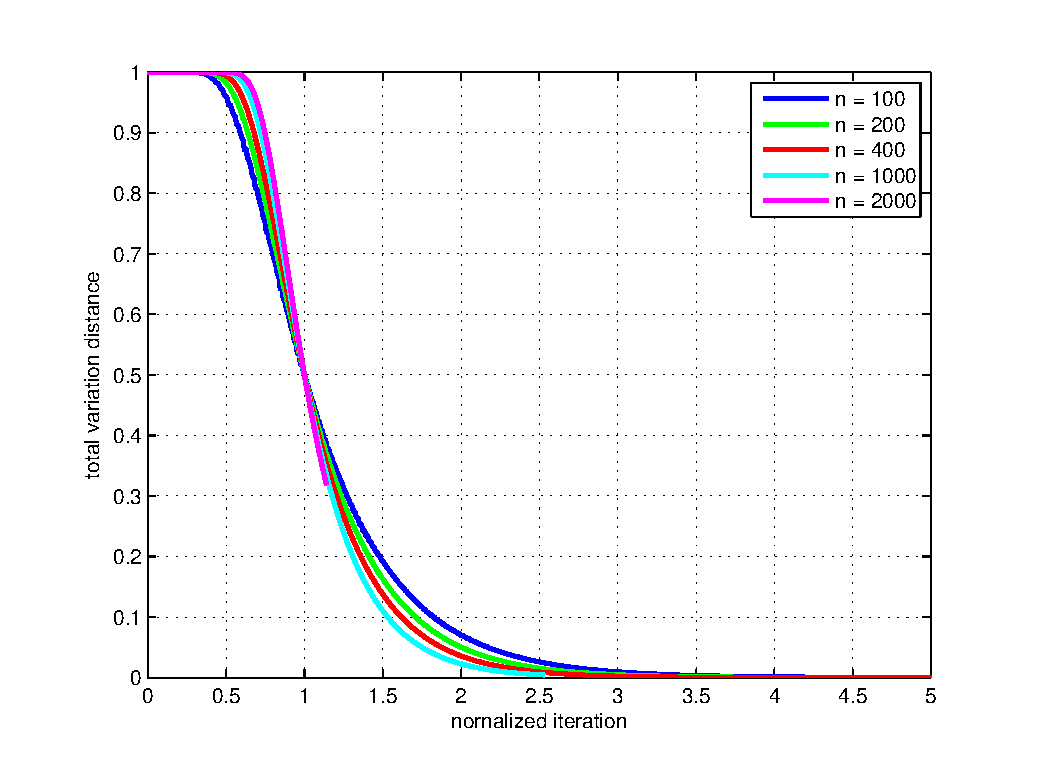
\includegraphics[width=0.4\hsize]{rdwalkn.eps} &
\begin{minipage}[b]{0.58\hsize}
The top figure shows $\|\omega^k - \bar{\omega}\|_{TV}$ versus $k$ trajectories for $n$ varying from $100$ to $2000$. In the bottom figure we normalize all the trajectories by scaling the $x$-axis and making all of the them pass through $(1, 0.5)$. The normalized trajectories become sharper and sharper when $n$ increases, so we conclude that this family $(\Omega_n,\bar{\omega}_n, (\omega^k_n)_{k=0,1,...})_{n=1,2,...}$ presents a total variation-cutoff.
\end{minipage}
\end{tabular}

\end{example}


%section ends here
%%%%%%%%%%%%%%%%%%%%%%%%%%%%%%%%%%%%%%%%%%%%%%%%%%%%%%%%%%%%%%%%%%%%%%%%%%%%%%%%%%%%%%%%%%%%%%%%%





}
\end{pcolumn}
\begin{pcolumn}{0.32}
%%%%%%%%%%%%%%%%%%%%%%%%%%%%%%%%
%Here is the 2nd column
%%%%%%%%%%%%%%%%%%%%%%%%%%%%%%%%
\pbox{0.9\textwidth}{65cm}{linewidth=4mm,framearc=0.1,linecolor=red,fillstyle=gradient,gradangle=0,gradbegin=white,gradend=white,gradmidpoint=1.0,framesep=1em}{



\begin{center}\pbox{0.8\textwidth}{}{linewidth=2mm,framearc=0.1,linecolor=red,fillstyle=gradient,gradangle=0,gradbegin=white,gradend=whitered,gradmidpoint=1.0,framesep=1em}{\begin{center}\bfseries{\large{Tent Map and Logistic Map Cutoffs}}\end{center}}\end{center}\vspace{1cm}

%%%%%%%%%%%%%%%%%%%%%%%%%%%%%%%%%%%%%%%%%%%%%%%%%%%%%%%%%%%%%%%%%%%%%%%%%%%%%%%%%%%%%%%%%%%%%%%%
%Section begins here

\begin{tabular}{c|l}
  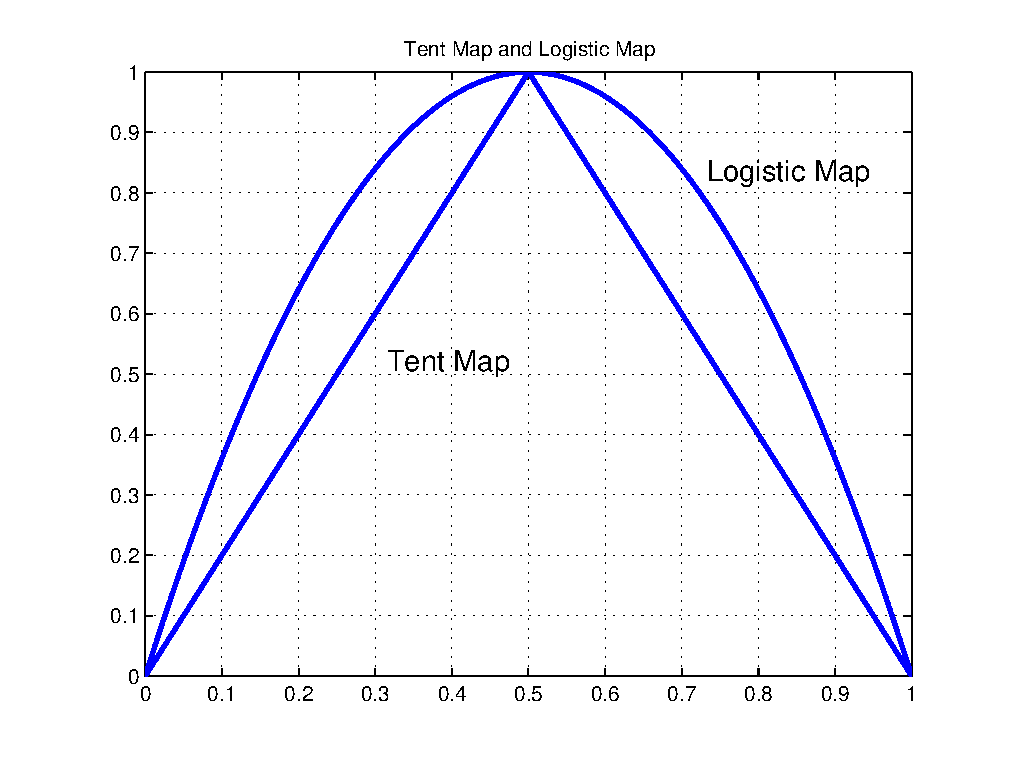
\includegraphics[width=0.35\hsize]{tentmapandlogisticmap.eps}&
  \begin{minipage}[b]{0.6\hsize}
    \textbf{Tent Map}  
     \begin{eqnarray}
        \label{tentmap}
          x' = S_\text{tent}(x) \equiv 1-2|x-\frac{1}{2}|
     \end{eqnarray}
    \textbf{Logistic Map}
     \begin{eqnarray}
        \label{logisticmap}
          x' = S_\text{logistic}(x) \equiv rx(1-x)
     \end{eqnarray}
    Both are known to be chaotic. 
  \end{minipage}
\end{tabular}


\vspace{0.4cm}
Let $X = [0,1]$ and $\nu$ be the Borel measure. In the measure space  $(X,\mathcal{A},\nu)$, for a given 1-D map $S: X \rightarrow X $ with $\bar{\omega}(S^{-1}(A))=\bar{\omega}(A)$ for all $A \in \mathcal{A}$. The probability measure $\omega$  is transported by $S$ in the following way, 
  \begin{eqnarray}
  \label{omegamap}
    \omega'(x') = \sum_i \left|\frac{dx_i}{dx'}\right|\omega(x) \mbox{   , for all } i \mbox{  such that  } x'=S(x_i)
  \end{eqnarray}
Consider the following initial distribution on $[0 ,1]$
  \begin{eqnarray}
  \label{tentmapinitial}
    \omega_{\mu_n}^0 = \left\{ \begin{tabular}{c}
                      $\frac{1}{\mu_n}$, \mbox{  if  } $x \le \mu_n$\\ 
                      $0$, \mbox{  otherwise} 
                      \end{tabular}\right.
  \end{eqnarray}
where $\mu_1 = 1$, and $\mu_{n+1} = \frac{\mu_n}{2}$ for the tent map and $\mu_{n+1}=\frac{1-\sqrt{1-\mu_n}}{2}$ for the logistic map. By applying (\ref{omegamap}), their Perron-Frobenius operators are,
  \begin{eqnarray}
  \label{tentmapevolve}
    \omega_{\mu_n}^{k+1}(x) \equiv P_\text{tent} \omega_{\mu_n}^{k}(x)
                             = \frac{1}{2}\left( \omega_{\mu_n}^{k}\left(\frac{x}{2}\right)+
                                                 \omega_{\mu_n}^{k}\left(1-\frac{x}{2}\right)  \right)
  \end{eqnarray}
 \begin{eqnarray}
 \label{logisticmapevolve}
    \omega_{\mu_n}^{k+1}(x) &\equiv &P_\text{logistic} \omega_{\mu_n}^{k}(x) \nonumber\\
                            &     = &\frac{1}{4\sqrt{1-x}}\left( \omega_{\mu_n}^{k}\left( \frac{1-\sqrt{1-x}}{2}\right)
                                            +\omega_{\mu_n}^{k}\left( \frac{1+\sqrt{1-x}}{2}\right) \right)
 \end{eqnarray}
We have the following two theorems

\begin{theorem} {\bfseries (Tent map cutoff)}
The family $([0,1],\bar{\omega}, (\omega^k_{\mu_n})_{k=0,1,...})_{n=1,2,...}$, where $\bar{\omega}$ is uniform in $[0,1]$ and $\omega^k_{\mu_n}$ are defined as in (\ref{tentmapinitial}) and (\ref{tentmapevolve}), presents a Total Variation-cutoff in the relaxed sense.
\end{theorem}

\begin{theorem} {\bfseries (Logistic map cutoff)}

The family $([0,1],\bar{\omega}, (\omega^k_{\mu_n})_{k=0,1,...})_{n=1,2,...}$, where $\bar{\omega}= \frac{1}{\pi\sqrt{x(1-x)}}$ and $\omega^k_{\mu_n}$ are defined as in (\ref{tentmapinitial}) and (\ref{logisticmapevolve}), presents a Total Variation-cutoff between $k=n-1$ and $n$ in the relaxed sense .
\end{theorem}




\begin{center}
  \includegraphics[width=0.32\hsize]{tentmapcutoff.eps}
  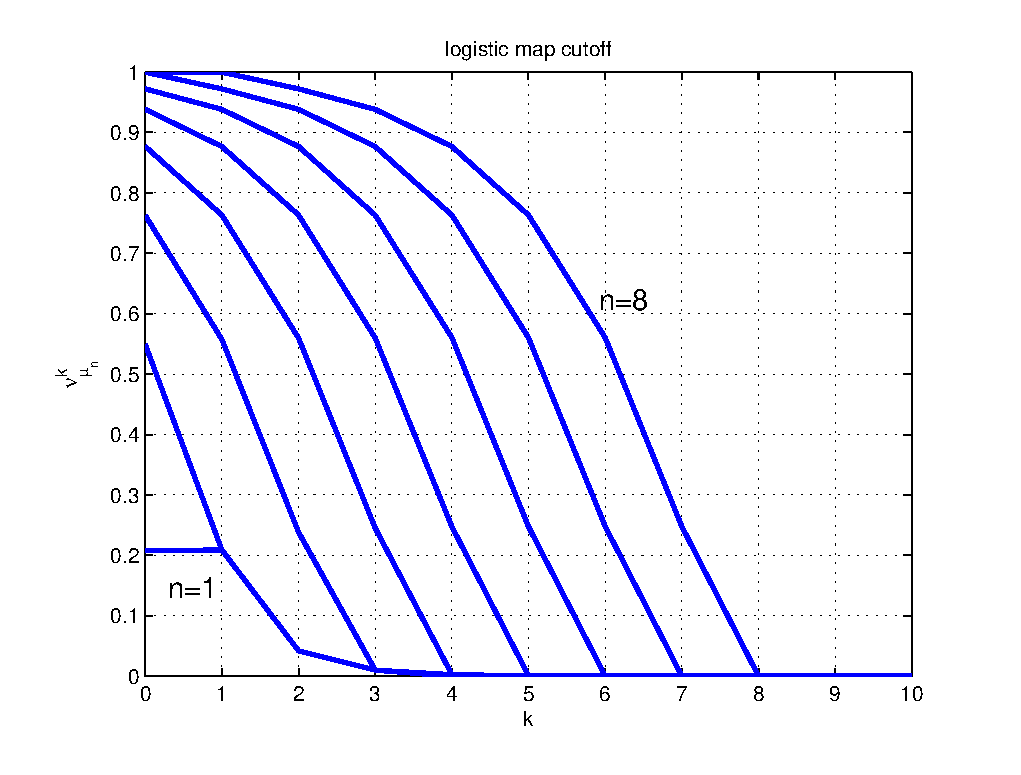
\includegraphics[width=0.32\hsize]{logisticmapcutoff.eps}
  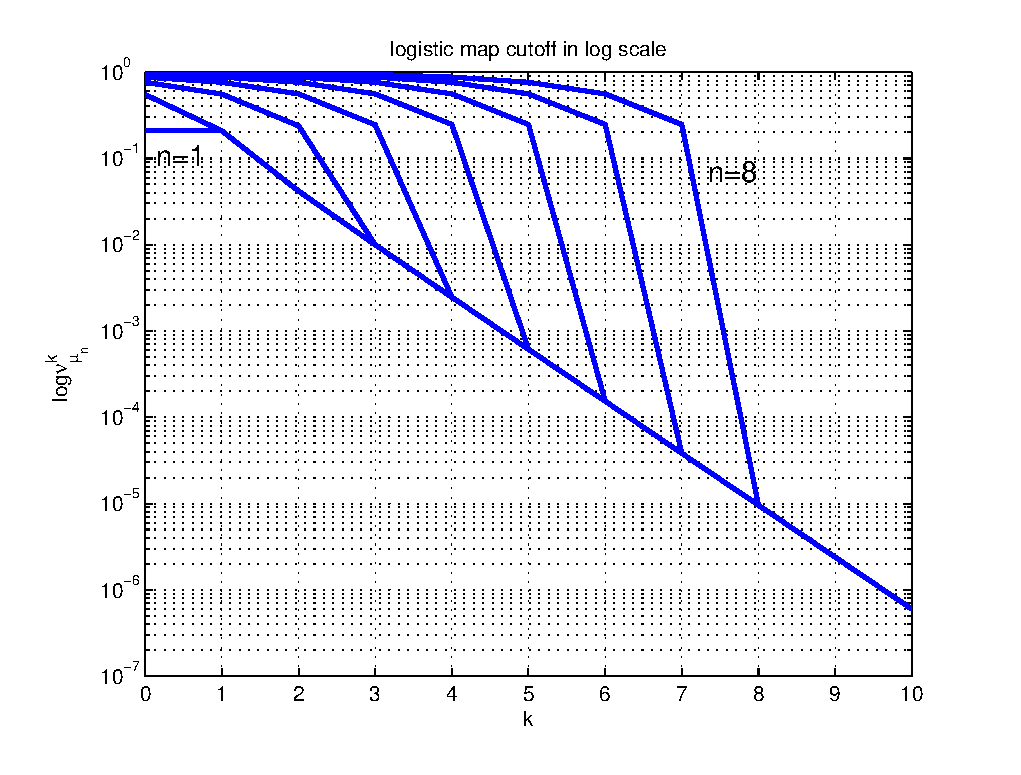
\includegraphics[width=0.32\hsize]{logisticmapcutofflog.eps}
\end{center}

\begin{tabular}{c|l}
   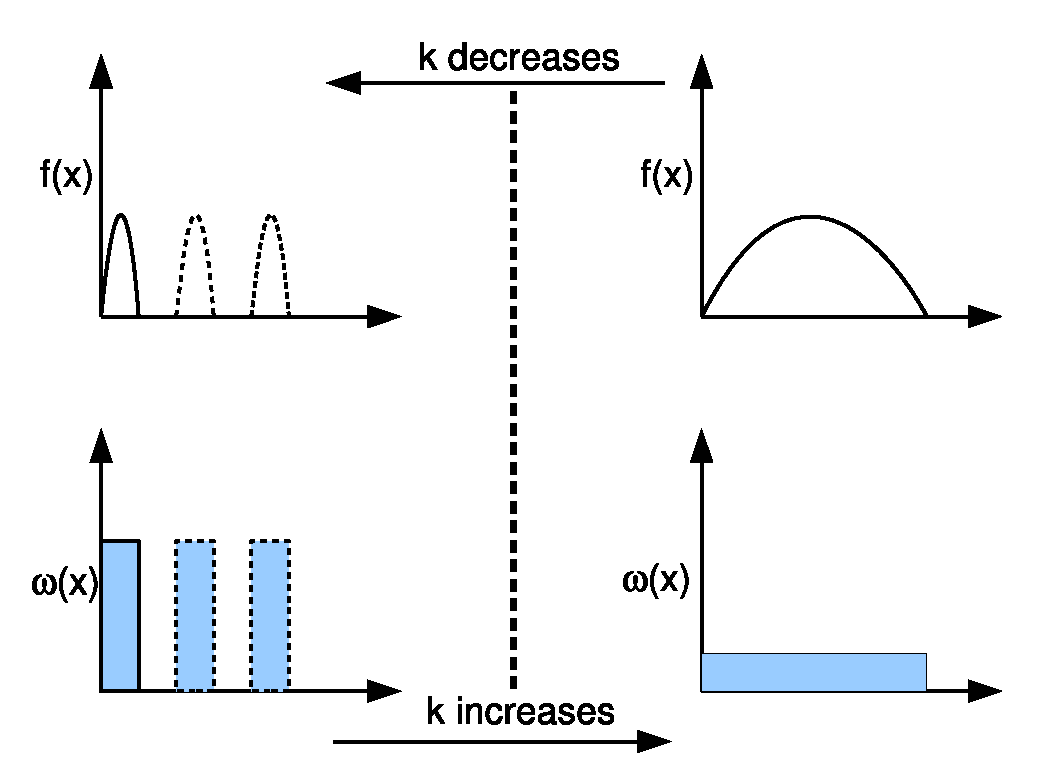
\includegraphics[width=0.4\hsize]{cutoffexplain.eps}&
   \begin{minipage}[b]{0.5\hsize}
\paragraph{The relation between $\omega^k$ and $f^k$}
One feature of unimodal maps is that a non-vanishing $\omega^k$ can have many possible histories (many different $\omega^0$). For a scalar function $f^k$ carried by the probability density $\omega^k$, they satisfy $(f^{k+1})^T\omega^{k+1}=(f^k)^T\omega^k$. This implies that if we evolve a simple function by the map backwards in time, each of the possible $\omega^0$s needs to contain the same information as $f^k$. Hence it results in a frequency cascade.   
   \end{minipage}
\end{tabular}

}
\end{pcolumn}
\begin{pcolumn}{0.32}
%%%%%%%%%%%%%%%%%%%%%%%%%%%%%%%%
%Here is the 3rd column
%%%%%%%%%%%%%%%%%%%%%%%%%%%%%%%%
\pbox{0.9\textwidth}{65cm}{linewidth=4mm,framearc=0.1,linecolor=red,fillstyle=gradient,gradangle=0,gradbegin=white,gradend=white,gradmidpoint=1.0,framesep=1em}{

\begin{center}\pbox{0.8\textwidth}{}{linewidth=2mm,framearc=0.1,linecolor=red,fillstyle=gradient,gradangle=0,gradbegin=white,gradend=whitered,gradmidpoint=1.0,framesep=1em}{\begin{center}\bfseries{\large{Cutoff in Advection-Diffusion Simulation}}\end{center}}\end{center}\vspace{1.25cm}

%%%%%%%%%%%%%%%%%%%%%%%%%%%%%%%%%%%%%%%%%%%%%%%%%%%%%%%%%%%%%%%%%%%%%%%%%%%%%%%%%%%%%%%%%%%%%%%%
%Section begins here
The following table shows the relation between Perron-Frobenius and Koopman operators.

\vspace{0.4cm}
\centerline{
\begin{tabular}{l|cc}
                      & forward in time                    & backward in time     \\
\hline
        probability measure & $P_S$, $(A^T)$                       &  $P_{S^{-1}}$, $(B^T)$  \\
        function            & $P_{S^{-1}}^* = U_{S^{-1}}$, $(B)$ &  $P_S^* = U_S $, $(A)$ 
\end{tabular}
}
\vspace{0.4cm}

We are now going to study the Koopman operator of \textbf{Standard Map},
  \begin{eqnarray}
               x_1' &=&  x_1+x_2 +\epsilon \sin{2 \pi x_1} (\mbox{ mod } 1) \nonumber\\
               x_2' &=&  x_2 +\epsilon \sin{2 \pi x_1}     (\mbox{ mod } 1)
  \end{eqnarray}
with added diffusion. A sequence of $A_n \in \mathbb{R}^{n^2}$ such that $\lim_{n \rightarrow \infty} A_n = A$ are generated. They correspond to a sequence of approximated Koopman operators of Standard Map with decreasing numerical diffusion, or ascending accuracy. Then we simulate this sequence of linear systems with initial function  $f_n^{\infty} = g_n(\cos(2 \pi x_2))$, where $g_n$ discretizes $\cos(2 \pi x_2)$ in the space $\mathbb{R}^{n^2}$.



\begin{tabular}{c|c}
   \includegraphics[width=0.65\hsize]{demostandardmapcos.eps}&

   \begin{minipage}[b]{0.33\hsize}
    The simulation of $f_n^k = A_n f_n^{k+1}$ with $n = 1000$, $k = 0,2,5,10,20$ and $30$. The colors are mixed quickly in the chaotic region even when the diffusion is small. The bottom figure shows the same simulation without numerical diffusion.    
    
 \centerline{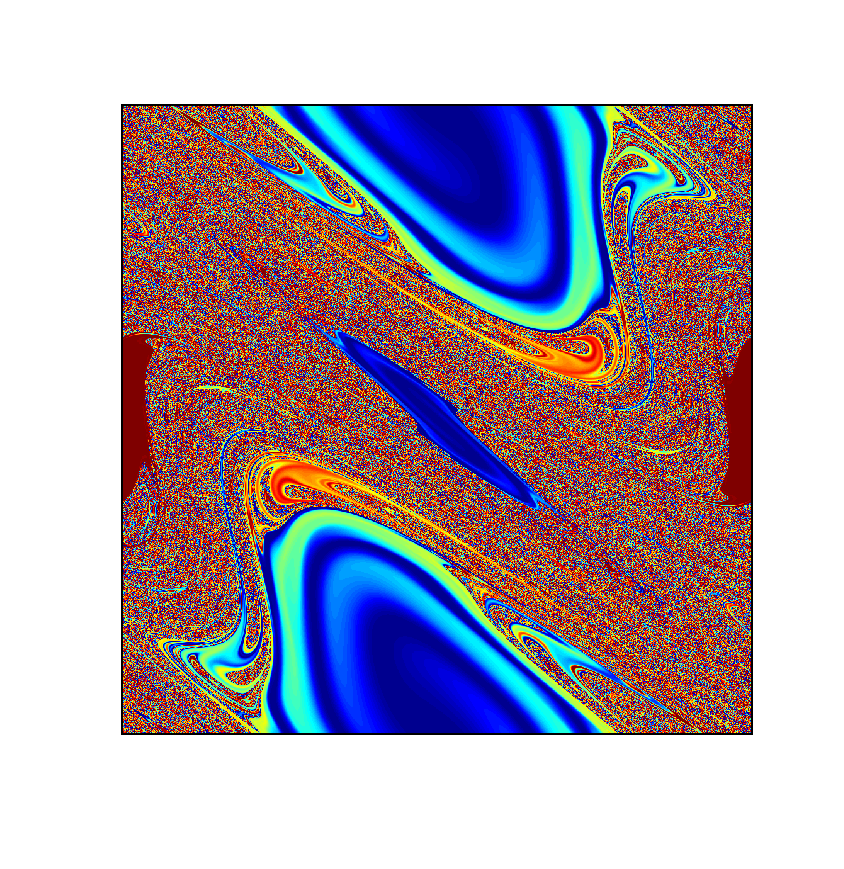
\includegraphics[scale=0.6,angle=90]{standardmapsimuexact2.eps}}
   \end{minipage} 
\end{tabular}

\begin{tabular}{cc|l}
   
        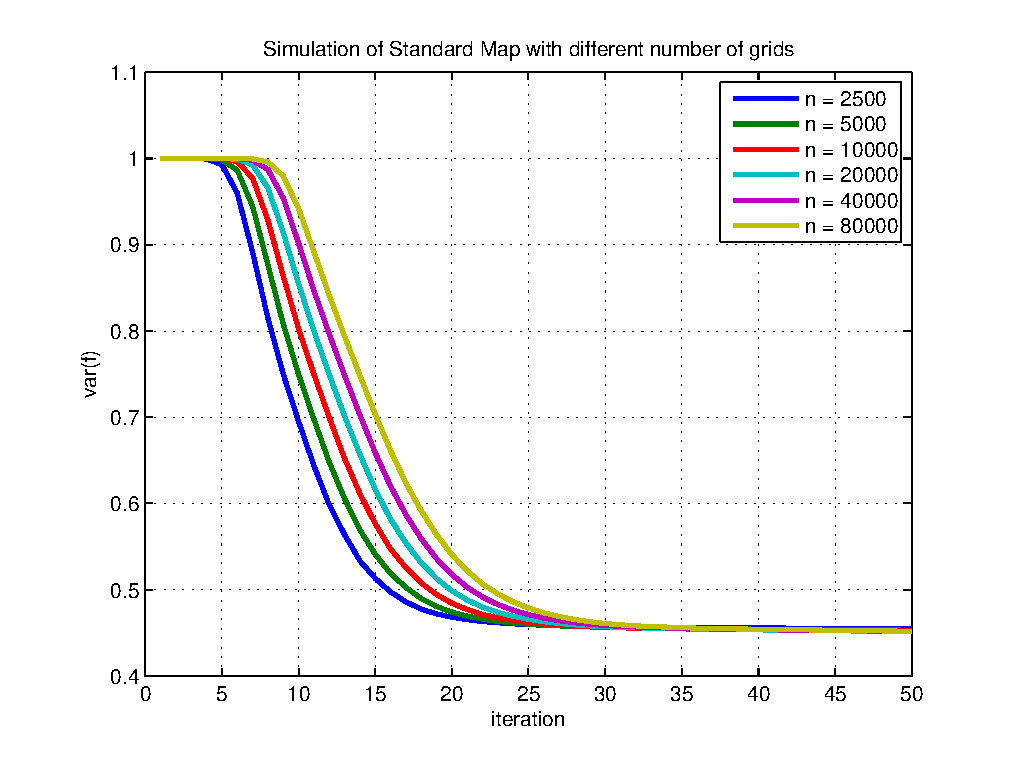
\includegraphics[width=0.35\textwidth,trim=0cm 0cm 0cm 0cm]{standardmapcutoff}&
	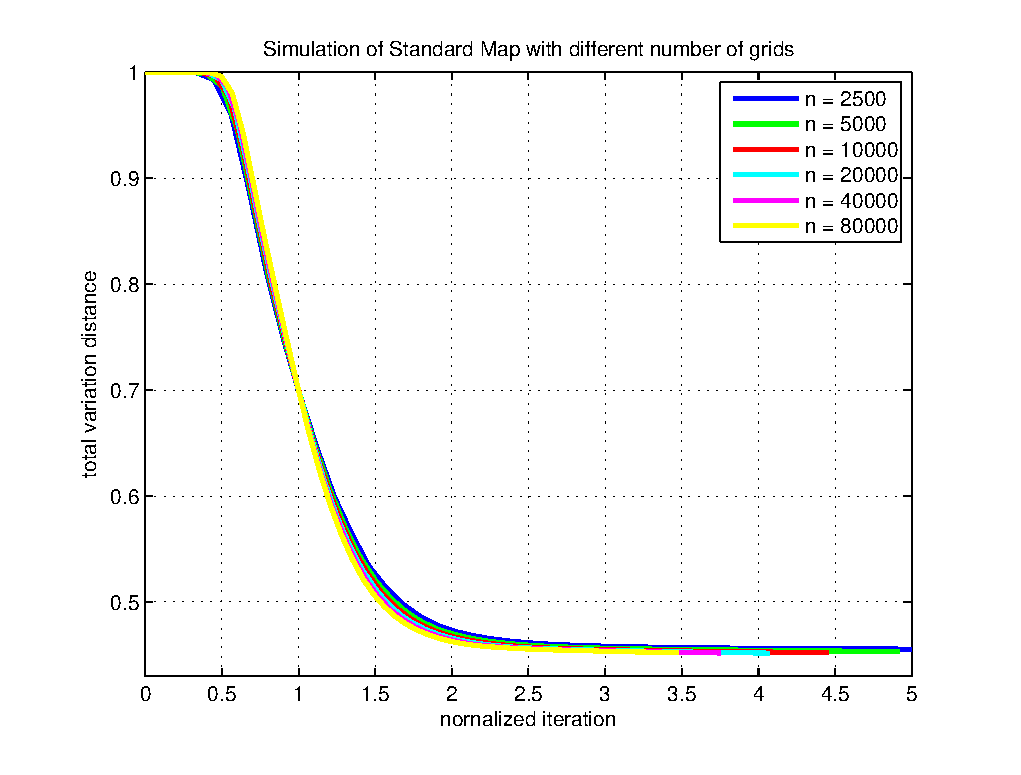
\includegraphics[width=0.35\textwidth,trim=0cm 0cm 0cm 0cm]{standardmapcutoffn}&
   \begin{minipage}[b]{0.28\hsize}
    Now with $n$ varying from $2500$ to $80000$, the total variation versus iteration plot is shown in the left figure. The  trajectories are normalized and plotted again in the right figure. They present a cutoff.
    \end{minipage} 
\end{tabular}









%Section ends here
%%%%%%%%%%%%%%%%%%%%%%%%%%%%%%%%%%%%%%%%%%%%%%%%%%%%%%%%%%%%%%%%%%%%%%%%%%%%%%%%%%%%%%%%%%%%%%%%

% Future Work
\begin{center}\pbox{0.8\textwidth}{}{linewidth=2mm,framearc=0.1,linecolor=red,fillstyle=gradient,gradangle=0,gradbegin=white,gradend=whitered,gradmidpoint=1.0,framesep=1em}{\begin{center}\bfseries{\large{Future Work}}\end{center}}\end{center}\vspace{0.5cm}

%We prove that tent map and logistic map both present cutoffs when suitable sequence of initial probability distributions are chosen. We also numerically demonstrate that a similar cutoff can be observed when a passive scalar function is advected by the chaotic map with small diffusion. The above two findings show that phase change appears in both chaotic randomizing and chaotic mixing problems.   
\begin{itemize}
\item Explore the cutoffs of other measures of cetrainty/uncertainty besides total variation. 
\item Do cutoffs shown in chaotic mixing and chaotic randomizing imply each other?
\item Define a measure of chaos through cutoff. 
\end{itemize}

\vspace{-0.5cm}
% References
\bibliographystyle{plain}
\bibliography{mixingbib}
\nocite{Thiffeault2004}
\nocite{Mezic2005}

}
\end{pcolumn}
\end{center}



\vspace*{2cm}



\end{poster}

\end{document}

